\documentclass[12pt,letterpaper]{article}
\usepackage[utf8]{inputenc}

%Documento
\usepackage[spanish,es-tabla,es-lcroman]{babel}
\usepackage[T1]{fontenc}
\usepackage{times}
\usepackage[margin=2.54cm]{geometry}
\usepackage{parskip} %saltos de parrafo
\setlength{\parskip}{\baselineskip}

%Formatos
\usepackage{setspace} %espacios de interlineados
\usepackage[dvipsnames]{xcolor} %paquete para colores
%tablas
\usepackage{array}
\usepackage{multicol}
\usepackage{longtable}

%imagenes
\usepackage{graphicx}
\usepackage{subcaption}
\usepackage{enumerate} %numeracion de tablas y figuras
%Listas
\usepackage[shortlabels]{enumitem}

%hipervinculos
\usepackage{hyperref}%Genera hipervinculos
\hypersetup{colorlinks=true,citecolor=black,filecolor=black,linkcolor=black,urlcolor=blue}

%Referencias
\usepackage{natbib}

%matematicas
\usepackage{amsmath,amssymb,amsfonts}

% - - - - - - - - - - - - - - - - - - - - - - - - - - - - - - - - - - - - - - - - - - - - - - 
%Indice de ecuaciones, figuras y tablas
\numberwithin{equation}{section} 	
\numberwithin{figure}{section}
\numberwithin{table}{section}

\begin{document}
\begin{titlepage}
    \begin{center}
        \noindent 
\includegraphics[width=\textwidth]{Imagenes/logos latex.PNG} \\[2cm] %el noident fue para quitar la sangria... texwidht es para que la imagen sea del ancho de la pagina 
        \textbf{{\Huge CENTRO NACIONAL DE INVESTIGACIÓN Y DESARROLLO TECNOLÓGICO}}\\[1cm]
        
        \textbf{\Large{Doctorado en Ciencias en Ingeniería Electrónica}}\\
        {\large Especialidad en Control Automático}\\[1cm]
        
        \textbf{{\Large Propuesta de tesis}}\\
        {\large 2° semestre}\\[1cm]
              
        \textbf{\Large{\textcolor{MidnightBlue}{Modelado de datos ómicos con técnicas de aprendizaje profundo mediante redes neuronales}}}\\[1cm]
        
        {\large Presenta:}\\
        \textbf{{\Large M.C. Arturo Figueroa Arcos}}\\[1cm]
    
    \end{center}
    \begin{minipage}{0.46\textwidth}								
        \begin{flushleft}
        \begin{center}
    
            \textbf{Directores de tesis:}\\
        
            Dr.\ Víctor Manuel Alvarado Martínez\
            Dra. Ma. Guadalupe López López\\
            
    \end{center}
    \end{flushleft}
    \end{minipage}		
                                                                    %%%
    \begin{minipage}{0.52\textwidth}		
    \vspace{0cm}
    \begin{flushright}															%%%
    \begin{center}
    
            \textbf{Revisores de tesis:}\\
    
            Dr.\ Luis Gerardo Vela Valdés\\
            Dr.\ Victor Hugo Olivares Peregrino\\
            Dra. Marisol Cervantes Bobadilla\\
    
            
    \end{center}
    \end{flushright}
    \end{minipage}	
    \vspace*{3cm}
    
    \begin{flushright}
    {\large Cuernavaca, Morelos a 06 de diciembre de 2024}
    \end{flushright}
    
    \end{titlepage}
\pagenumbering{roman}
\renewcommand{\contentsname}{Tabla de contenido}
\tableofcontents
\newpage

\newpage
\listoffigures
\addcontentsline{toc}{section}{Índice de figuras}

\newpage
\listoftables
\addcontentsline{toc}{section}{Índice de tablas}

\newpage
\addcontentsline{toc}{section}{Nomenclatura}

% - - - - - - - - - - - - - - - - - - -- - - - - - - - - - - - - - - - - - - - - - - -- - - - -
%Nomenclatura

\textbf{\Large{Nomenclatura}}

\begin{table}[h]

    \centering
    \caption{Siglas y acrónimos}
    \vspace{0.3cm}
    \begin{tabular}{
    >{\centering\arraybackslash}m{3cm}
    >{\centering\arraybackslash}m{12cm}} \hline

\textbf{Siglas} & 
\textbf{Descripción} \\ \hline\hline

   IA & Inteligencia Artificial
\\[0.2cm]

   DL & Aprendizaje Profundo (En inglés Deep Learning)
\\[0.2cm]

   ML & Aprendizaje Automático (En inglés Machine Learning)
\\[0.2cm]

   CNN & Red Neuronal Convolucional (En inglés Convolutional Neuronal Network)
\\[0.2cm]
   RNN & Red Neuronal Recurrente (En inglés Recurrent Neuronal Network)
\\[0.2cm]
   NGS & Secuenciación de nueva generación (En inglés Next Generation Sequencing) 
\\[0.2cm]
   ANN & Red Neuronal Artificial (En inglés Artificial Neuronal Network) 
\\[0.2cm]
TCGA & Programa del Atlas del Genoma del Cáncer (En inglés The Cancer Genome Atlas Program) 
\\[0.2cm]
AE & Auto Codificador (En inglés Auto Encoder) 
\\[0.2cm]
GAN & Red Generativa Antagónica (En inglés Generative Adversarial Network) 
\\[0.2cm]
DNN & Red Neuronal Densa (En inglés Deep Neural Network) 
\\[0.2cm]
MLP & Perceptrón Multicapa (En inglés Multilayer Perceptron) 
\\[0.2cm]



\hline
    \end{tabular}
\end{table}

\newpage

\setcounter{page}{1} %se reinicia el contador de la páginas después de la Tabla de contenido
\pagenumbering{arabic}

% - - - - - - - - - - - - - - - - - - - - - - - - - - - - - - - -
%Documento principal

\section{Introducción}

En la ingeniería biomédica se aplica tecnología de última generación, para la creación de dispositivos médicos y métodos que permitan contribuir al bienestar humano, para obtener una mejora en la compresión de los procesos biológicos que suceden en el ser humano. En este campo de estudio intervienen áreas como la ingeniería electrónica, la ingeniería mecánica, la medicina, la biología, la física, entre otros, considerando a la ingeniería biomédica como un campo interdisciplinario.

La generación de datos ómicos ha experimentado un crecimiento exponencial gracias a las tecnologías de secuenciación de alto rendimiento (NGS). Debido a la alta cantidad de datos existentes, se han impulsado métodos analíticos avanzados para interpretarle y extraer información biológica significativa. Los datos que se abarcan son de diferentes niveles de organización molecular, como el ADN, el ARN, las proteínas y metabolitos.

 Algunos ejemplos de estos datos ómicos son los genómicos que estudian el ADN incluyendo la secuencia, estructura y función, los datos transcriptómicos que estudian el ARN incluyendo su expresión, splicing y modificaciones, los datos proteómicos que estudian las proteínas, incluyendo su estructura, función e interacciones y los datos metabolómicos que estudian las moléculas pequeñas que interactúan en las reacciones químicas de la célula.

El análisis de este tipo de datos cuenta con el potencial para mejorar significativamente nuestra compresión de la salud y las enfermedades en un ser humano. Los pasos típicos son el preprocesamiento donde se realiza la limpieza y normalización de los datos con el fin de eliminar errores, control de calidad para identificar y eliminar posibles valores atípicos, análisis estadístico para identificar biomarcadores relevantes así como también modelos predictivos y de asociación y por último la interpretación de los resultados con sentido biológico.
Algunos de los desafíos que se presentan en el análisis son el alto volumen de datos, complejidad de los datos y la integración de tipo de datos, es por ello por lo que se considera un desafío computacional.

El Aprendizaje Profundo (DL) es un campo de la inteligencia artificial, que ha demostrado ser una herramienta poderosa para el análisis de datos complejos, está basado en la utilización de redes neuronales artificiales (ANN’s) con el fin de identificar patrones complejos, realizar análisis no lineales y modelar relaciones a partir de diferentes tipos de datos ómicos.

Las ANN’s y DL aplicadas en la ingeniería biomédica representan una oportunidad para los profesionales de la salud, ya que permiten realizar análisis más rápidos de grandes conjuntos de datos e información médica relevante, mejoras en los métodos de diagnóstico y pronostico de enfermedades, diseño de terapias personalizadas y mejoras para el bienestar humano. Los principales desafíos que se presentan son la necesidad de grandes conjuntos de datos para entrenamiento de las redes, la interpretabilidad de las redes neuronales para comprender su toma de decisiones y el requerimiento computacional para entrenamiento de las redes \citep{sarmiento2020aplicaciones}.

En este proyecto se enfocará con el propósito de clasificación de tipos y subtipos de fenotipos, así como también en el pronóstico de supervivencia, utilizando de manera preliminar datos ómicos centrados en el cáncer como los genómicos, transcriptómicos, proteómicos y metabolómicos. El área de oportunidad que se encuentra es en el preprocesamiento de datos y la codificación debido a la heterogeneidad de los datos procedentes de distintas bases que se encuentran de libre acceso. El propósito de este estudio estará dirigido en el estudio de algoritmos de aprendizaje profundo e implementarlos con enfoque de aplicación en el área biomédica con el fin de dar soporte en la precisión del diagnóstico y predicción de enfermedades.
\section{Objetivos}

\subsection{Objetivo general}
\begin{itemize}

   \addtolength{\itemsep}{-4mm} %con esto se ajusta el interlineado entre la lista
        \item Modelar datos genómicos, transcriptómicos y proteómicos utilizando técnicas de aprendizaje profundo, empleando redes neuronales de diseño propio, y configurar la salida del modelo para propósitos de clasificación y predicción, enfocados en el diagnóstico y pronostico del cáncer.

    \end{itemize}


\subsection{Objetivos específicos}

\begin{itemize}

   \addtolength{\itemsep}{-4mm} %con esto se ajusta el interlineado entre la lista
        \item Codificar datos genómicos, transcriptómicos y proteómicos para ser alimentados en las redes neuronales.
        \item Implementar redes neuronales convolucionada (CNN) y recurrente (RNN), y entrenarlas.
        \item Proponer y diseñar una red neuronal propia a partir de las dos anteriores.
        \item Configurar en cada caso la salida, para propósito de clasificación y predicción.
        \item Enfocar el modelado de las redes neuronales para fines biomédicos en diagnóstico y pronostico del cáncer.
        \item Validar los resultados con las bases de datos e incluyendo opinión de especialistas.
    \end{itemize}
\section{Marco Teorico}

\subsection{Redes Neuronales Graficas}

Las Redes Neuronales de grafos (GNN) son modelos de aprendizaje profundo en los cuales se procesan datos en representaciones de grafos o redes. Las GNN permiten aprovechar las relaciones que se codifican en los grafos para extraer características significativas y realizar tareas como la clasificación de nodos, la predicción de aristas (conexiones) y la inferencia a nivel de grafo. Este tipo de modelos aprende de las incrustaciones que capturen la informacion estructural del grafo como las características que se tengan en los nodos como se puede observar en la figura \ref{fig:GNN}

\begin{figure}[h!]
    \centering
    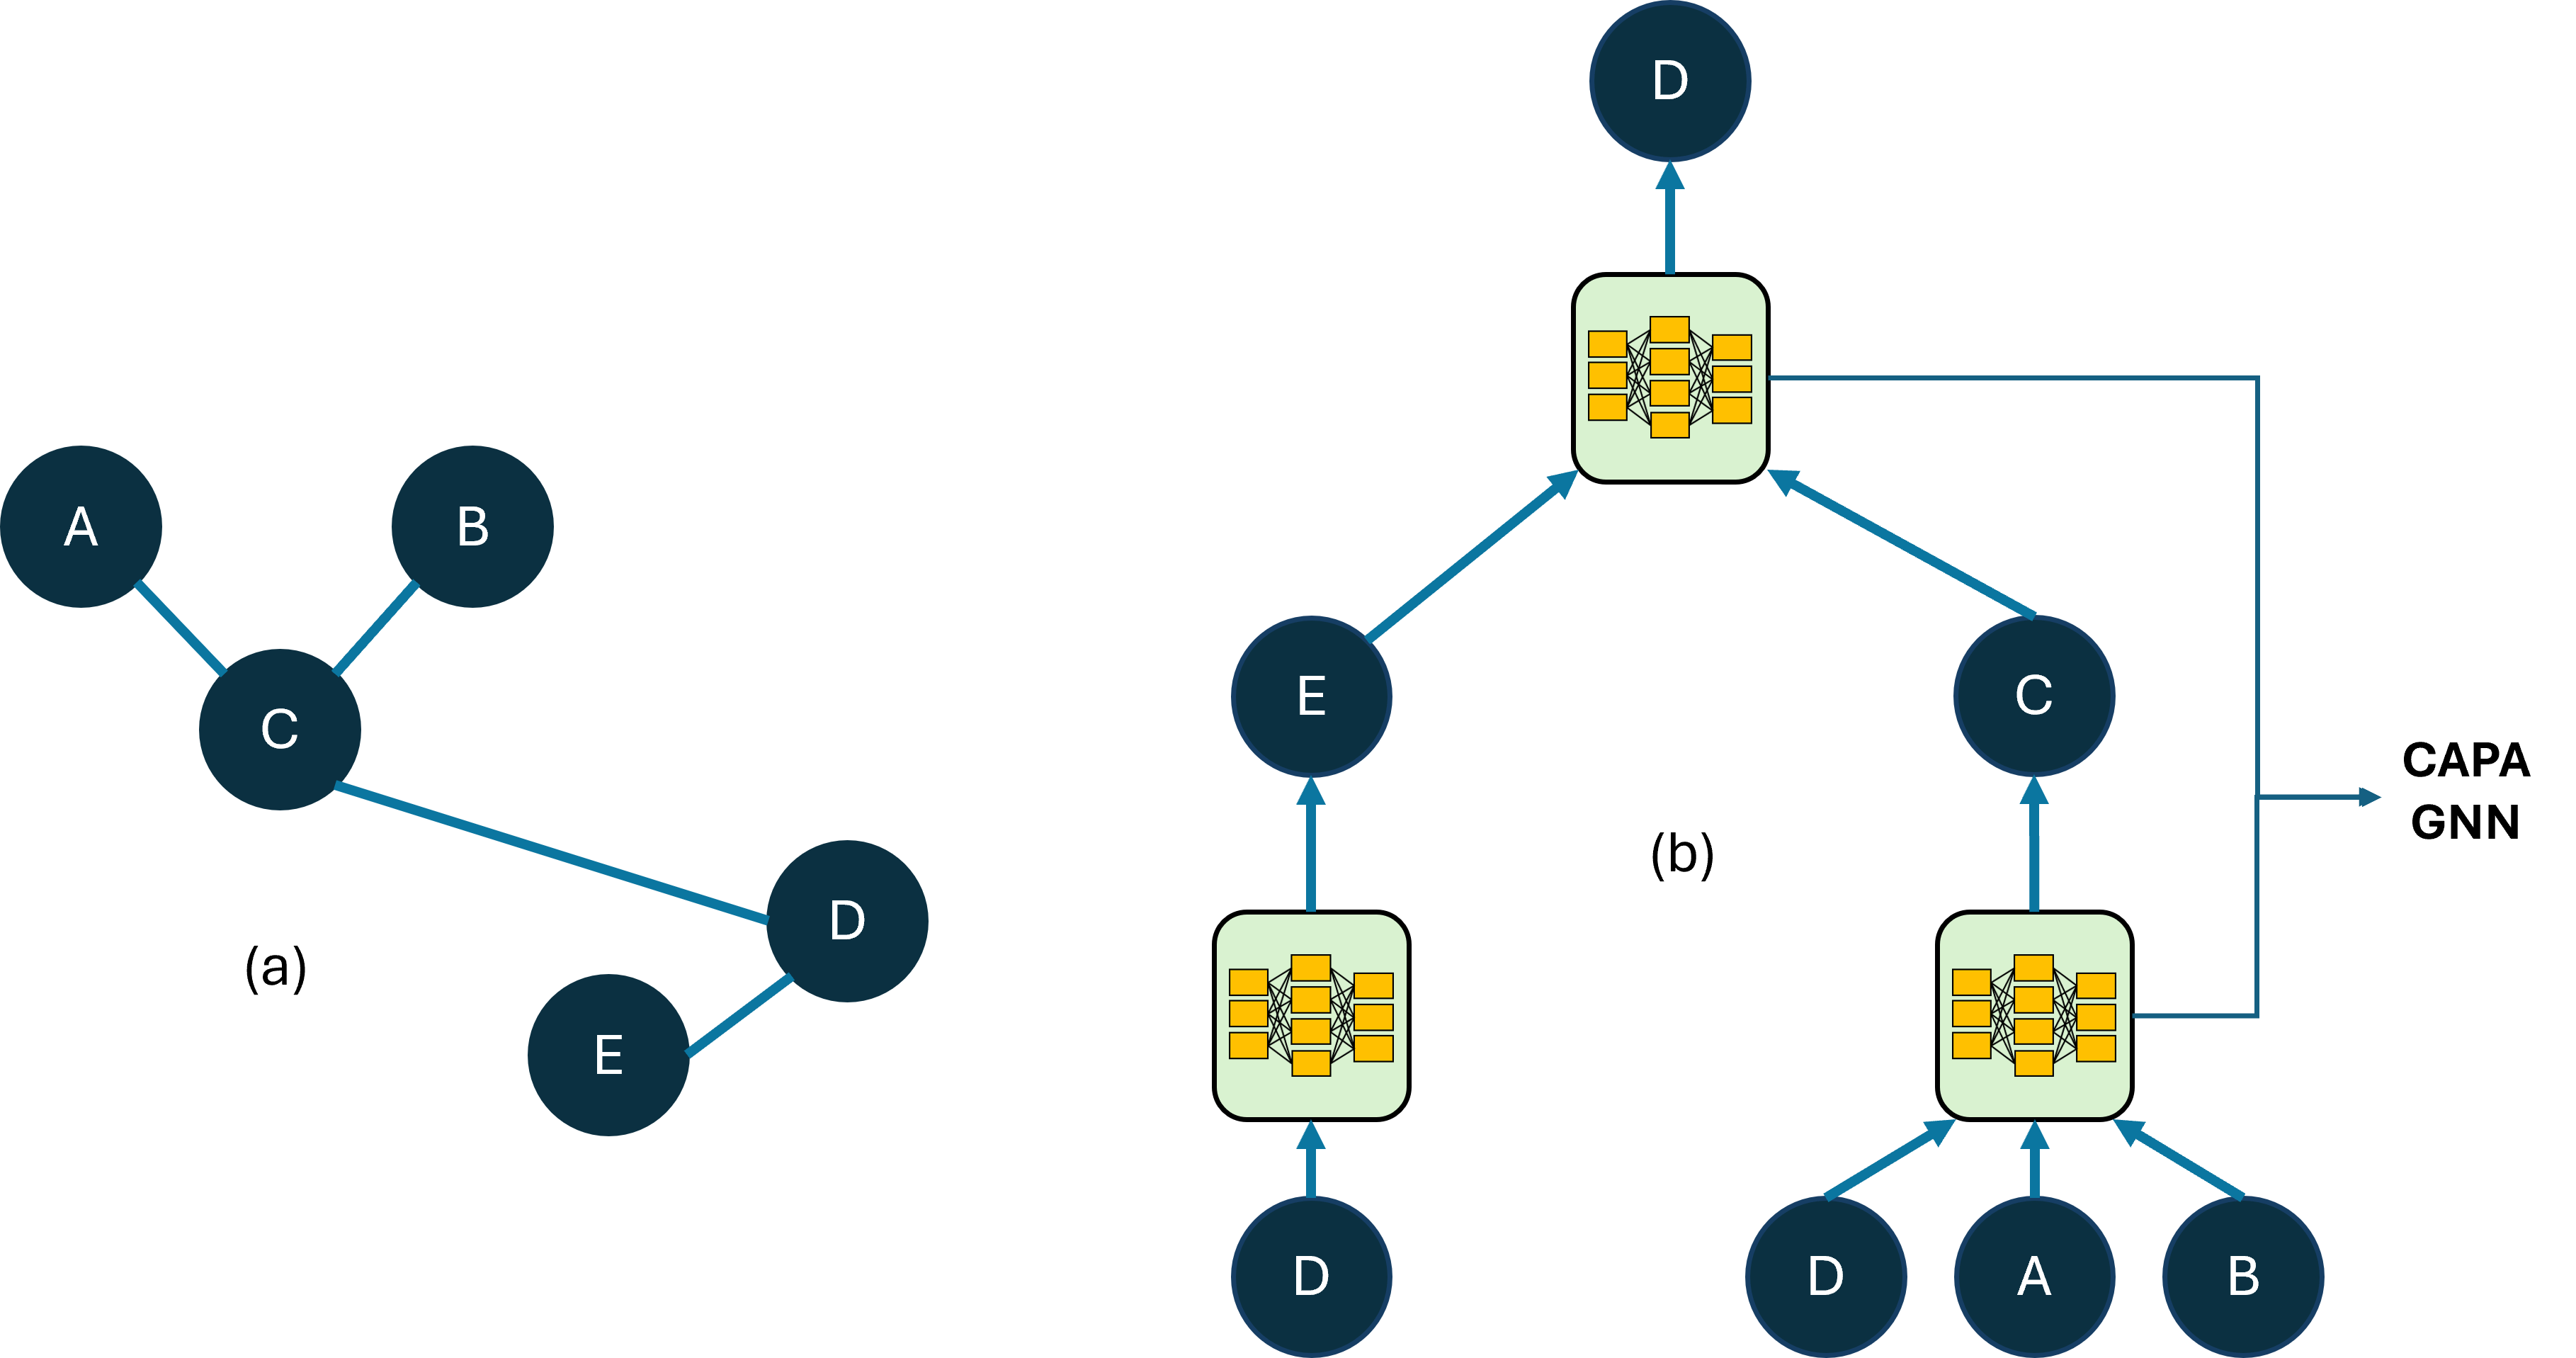
\includegraphics[width=0.9\textwidth]{Imagenes/GNN.png}
    \caption{Ilustración de grafo de entrada (a) y el proceso de la GNN en el cual se realiza el cálculo de la representación vectorial del nodo E agregando información de los nodos vecinos (b).}
    \label{fig:GNN}
\end{figure}

\subsubsection{Grafos}
\subsubsection{GAT}
\subsubsection{GCN}
\subsubsection{GTN}
\section{Avances}

\subsection{Procesamiento de datos ómicos}

\subsection{Estructuras DL en datos ómicos}
\section{Actividades futuras}
\section{Cronograma de actividades}

En esta sección se muestra es cronograma de las actividades que de manera preliminar se planean abordar los 4 años de estancia en CENIDET.

\begin{figure}[h!]
    \centering
    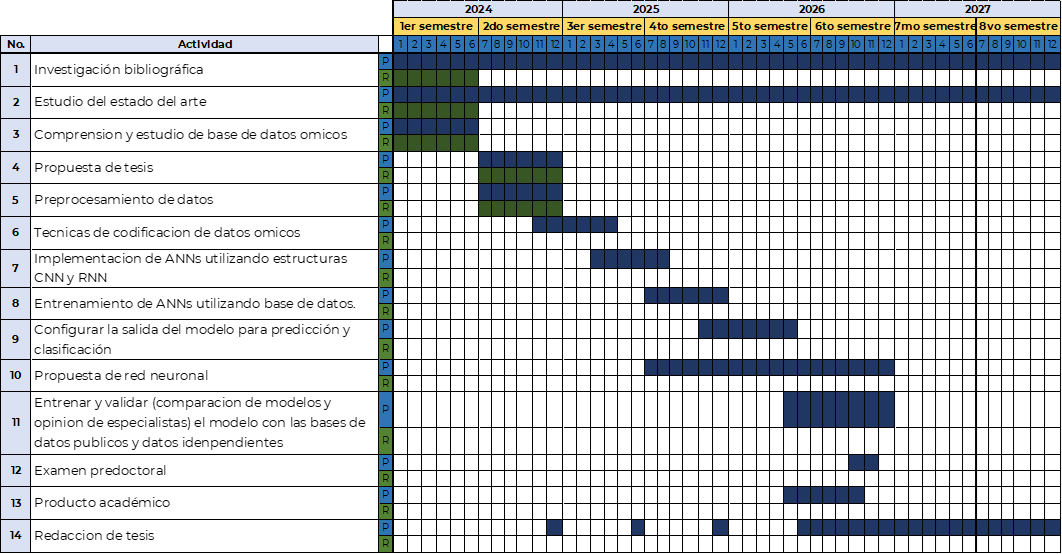
\includegraphics[width=1\textwidth]{Imagenes/Cronograma.png}
    \caption{Cronograma de actividades}\label{fig:cronograma}
\end{figure}


\newpage

\bibliographystyle{apalike} %eslito del citado %apacite %plain %apalike
\bibliography{bibliografia.bib} %archivo de las referencias

\end{document}